\documentclass[a4paper]{article}
\usepackage[margin=2cm]{geometry}

\usepackage{multirow}
 

\usepackage{polski}
\usepackage[utf8]{inputenc}
\usepackage[polish]{babel}

\usepackage{color, colortbl}
\usepackage[dvipsnames]{xcolor}
\usepackage{listings}
\usepackage{graphicx}

\usepackage{setspace}

\usepackage{natbib}

\lstset{literate=%
{ą}{{\k{a}}}1
{ć}{{\'c}}1
{ę}{{\k{e}}}1
{ł}{{\l{}}}1
{ń}{{\'n}}1
{ó}{{\'o}}1
{ś}{{\'s}}1
{ż}{{\.z}}1
{ź}{{\'z}}1
{Ą}{{\k{A}}}1
{Ć}{{\'C}}1
{Ę}{{\k{E}}}1
{Ł}{{\L{}}}1
{Ń}{{\'N}}1
{Ó}{{\'O}}1
{Ś}{{\'S}}1
{Ż}{{\.Z}}1
{Ź}{{\'Z}}1,
language=c++,
keywordstyle=\color{gray},
commentstyle=\color{lightgray},
stringstyle=\color{lightgray},
numbers=left,
frame=TBlr,
breaklines=true,
tabsize=2,
numberstyle=\tiny,
basicstyle=\footnotesize \ttfamily
}

\renewcommand\thesection{\arabic{section}.}
\renewcommand\thesubsection{\thesection\arabic{subsection}.}
\renewcommand\thesubsubsection{\thesubsection\arabic{subsubsection}.}
\renewcommand\theparagraph{\thesubsubsection\arabic{paragraph}.}
\renewcommand\thesubparagraph{\theparagraph\arabic{subparagraph}.}
\onehalfspacing
% Title Page
\title{Dokumentacja projektu  - inżynieria E-systemów w technologii JAVA \\ Aplikacja zarządzająca wydarzeniami kulturalnymi}
\author{\textbf{Przemysław Michalak} 181101\\ 
\textbf{Krystian Horecki} 181079 \\
\textbf{Grupa C} (śr. 11.15) \\ \\ Politechnika Wrocławska}
\date{20.05.2012 r.}

\begin{document}

\maketitle
\tableofcontents

\newpage


\section{Wymagania projektu}

Wymagania aplikacji zostały nieznacznie zmienione w miarę powstawania projektu.
Przy odpowiednich zmienionych wymaganiach zostały zamieszczone komentarze odnośnie zmienionych kryteriów oraz powodów takich zmian.

\subsection{Aplikacja internetowa}

\begin{table}[h!] 
\centering
\caption{Wymaganie funkcjonalne aplikacji internetowej FUN\_INT1}

\begin{tabular}{|p{2cm}|p{12cm}|} 

\hline	
	\multicolumn{2}{|>{\columncolor[gray]{.8}}c|}{Znajdowanie najbliższych wydarzeń	w sensie geograficznym}\\ \hline ID & FUN\_INT1 \\ 
	\hline \hline \multirow{2}{*}{Opis} & Użytkownik ma możliwość znalezienia wydarzeń  
	  znajdujących się najbliżej miejsca położenia podanego w aplikacji   \\	 
	\hline
	Priorytet & Wymagane \\ \hline	
	
\end{tabular}
\label{fun_int1}
\end{table}

Z uwagi na zmianę charakteru aplikacji, z nastawiania na wszelkie możliwe miejsca, na lokalizacje związane głównie z Wrocławiem, zrezygnowaliśmy z tej funkcjonalności.
Nie da się ukryć, iż implementacja posiadałaby duży nakład niepotrzebnej pracy.


\begin{table}[h!] 
\centering
\caption{Wymaganie funkcjonalne aplikacji internetowej FUN\_INT2}
\begin{tabular}{|p{2cm}|p{12cm}|} \hline	
	\multicolumn{2}{|>{\columncolor[gray]{.8}}c|}{Użytkownik ma możliwość dodawania wydarzeń}\\ \hline ID & FUN\_INT2 \\ \hline \hline
	 \multirow{2}{*}{Opis} &  Możliwe jest dodawanie przez użytkowników wydarzeń,   
	 które muszą być zatwierdzane przez administratora by mogły się pojawić 
	 w aplikacji, widoczne dla użytkowników \\
	 \hline Priorytet & Wymagane \\ \hline	
	
\end{tabular}
\label{fun_int2}
\end{table}

\begin{table}[h!] 
\centering
\caption{Wymaganie funkcjonalne aplikacji internetowej FUN\_INT3}
\begin{tabular}{|p{2cm}|p{12cm}|} \hline	
	\multicolumn{2}{|>{\columncolor[gray]{.8}}c|}{Przeglądanie wydarzeń}\\ \hline
	 ID & FUN\_INT3 \\ \hline \hline
	 \multirow{2}{*}{Opis} &  Aplikacja umożliwia przeglądanie wydarzeń według
	 wybranego kryterium (czas, miejsce, kategoria) \\  \hline 
	 Priorytet & Wymagane \\
	 \hline
	
\end{tabular}
\label{fun_int3}
\end{table}

W wypadku tej funkcjonalności uproszczony został system przeglądania wydarzeń, możliwe jest przeglądanie ich zgodnie z chronologią 
ich daty odbywania się, ma to związek z faktem braku odpowiedniego pola w bazie danych takiego jak kategoria wydarzenia, a także 
z uwagami zamieszczonymi odnośnie wymaganiem pierwszym.

\begin{table}[h!] 
\centering
\caption{Wymaganie funkcjonalne aplikacji internetowej FUN\_INT4}
\begin{tabular}{|p{2cm}|p{12cm}|} \hline	
	\multicolumn{2}{|>{\columncolor[gray]{.8}}c|}{Użytkownik ma możliwość podglądu miejsca wydarzenia}\\
	\hline ID & FUN\_INT4 \\ \hline \hline
	 \multirow{2}{*}{Opis} &  Aplikacja umożliwia uzyskanie podglądu na mapie
	 miejsca, w którym będzie odbywać się wydarzenie \\
	 \hline Priorytet & Wymagane \\
	 \hline
	
\end{tabular}
\label{fun_int4}
\end{table}

\begin{table}[h!] 
\centering
\caption{Wymaganie funkcjonalne aplikacji internetowej FUN\_INT5}
\begin{tabular}{|p{2cm}|p{12cm}|} \hline	
	\multicolumn{2}{|>{\columncolor[gray]{.8}}c|}{Aplikacja umożliwia załorzenie konta dla użytkownika}\\
	\hline ID & FUN\_INT5 \\ \hline \hline
	 \multirow{2}{*}{Opis} &  Możliwe jest założenie konta przez użytkownika,
	  oraz jego aktywacja poprzez email. \\
	  \hline Priorytet & Wymagane \\ \hline
	
\end{tabular}
\label{fun_int5}
\end{table}

W celu ułatwienia dostępu dla użytkowników walidacja konta odbywa się poprzez captche, a nie jak początkowo zakładano poprzez email.


\begin{table}[h!] 
\centering
\caption{Wymaganie funkcjonalne aplikacji internetowej FUN\_INT6}
\begin{tabular}{|p{2cm}|p{12cm}|} \hline	
	\multicolumn{2}{|>{\columncolor[gray]{.8}}c|}{Aplikacja umożliwia użytkownikowi dodawanie wydaerzeń do obserwowanych }\\ 
	\hline ID & FUN\_INT6 \\ \hline
	 \hline \multirow{2}{*}{Opis} &  Możliwe jest dodawanie przez użytkownika 
	 wydarzeń do ulubionych, a następnie ich podgląd na stronie konta użytkownika.
	 \\ \hline Priorytet & Wymagane
	 \\
	 \hline
	
\end{tabular}
\label{fun_int6}
\end{table}
\pagebreak
\subsection{Aplikacja mobilna}

\begin{table}[h!] 
\centering
\caption{Wymaganie funkcjonalne aplikacji mobilnej FUN\_MOB1}
\begin{tabular}{|p{2cm}|p{12cm}|} \hline	
	\multicolumn{2}{|>{\columncolor[gray]{.8}}c|}{Aplikacja umożliwia wyświetlenie wydarzeń }\\
	\hline ID & FUN\_MOB1 \\ \hline
	 \hline \multirow{2}{*}{Opis} &  Aplikacja umożliwia użytkownikowi wyświetlenie
	 wydarzeń na ekranie telefonu komórkowego. 
	 Możliwy jest określenie zakresu wyświetlania według kategorii, miejsca i
	 czasu. \\ 
	 \hline Priorytet & Wymagane
	 \\
	 \hline
	
\end{tabular}
\label{fun_mob1}
\end{table}

Uwagi identyczne jak odnośnie analogicznego wymagania dla aplikacji internetowej.

\begin{table}[h!] 
\centering
\caption{Wymaganie funkcjonalne aplikacji mobilnej FUN\_MOB2}
\begin{tabular}{|p{2cm}|p{12cm}|} \hline	
	\multicolumn{2}{|>{\columncolor[gray]{.8}}c|}{Aplikacja umożliwia zalogowanie się użytkownika }\\
	\hline ID & FUN\_MOB2 \\ \hline
	 \hline \multirow{2}{*}{Opis} &  Użytkownik ma możliwość zalogowania się do
	 aplikacji, co daje mu więcej funkcjonalności (dodawanie wydarzeń do
	 ulubionych). \\ \hline Priorytet & Wymagane
	 \\
	 \hline
	
\end{tabular}
\label{fun_mob2}
\end{table}

\begin{table}[h!] 
\centering
\caption{Wymaganie funkcjonalne aplikacji mobilnej FUN\_MOB3}
\begin{tabular}{|p{2cm}|p{12cm}|} \hline	
	\multicolumn{2}{|>{\columncolor[gray]{.8}}c|}{Aplikacja umożliwia dodawanie	wydarzeń do ulubionych }\\ 
	\hline ID & FUN\_MOB3 \\ \hline
	 \hline \multirow{2}{*}{Opis} & Użytkownik po zalogowaniu się, ma
	 możliwość dodawania wydarzeń do ulubionych. \\
	 \hline Priorytet & Wymagane
	 \\
	 \hline
	
\end{tabular}
\label{fun_mob3}
\end{table}


\begin{table}[h!] 
\centering
\caption{Wymaganie funkcjonalne aplikacji mobilnej FUN\_MOB4}
\begin{tabular}{|p{2cm}|p{12cm}|} \hline	
	\multicolumn{2}{|>{\columncolor[gray]{.8}}c|}{Aplikacja umożliwia poprowadzenie	użytkownika do miejsca wydarzenia}\\
	 \hline ID & FUN\_MOB4 \\ 
	\hline \hline
	 \multirow{2}{*}{Opis} &  Użytkownik po wybraniu wydarzenia ma możliwość
	 uzyskania widoku mapy, wraz z podaną trasą od miejsca aktualnego położenia
	 do miejsca w którym odbywa się wydarzenie.\\ 
	 \hline Priorytet & Wymagane
	 \\
	 \hline
	
\end{tabular}
\label{fun_mob4}
\end{table}
\pagebreak
\section{Wymagania niefunkcjonalne}
\subsection{Aplikacja internetowa}
\begin{table}[h!] 
\centering
\caption{Wymaganie niefunkcjonalne aplikacji internetowej NFUN\_INT1}
\begin{tabular}{|p{2cm}|p{12cm}|} \hline	
	\multicolumn{2}{|>{\columncolor[gray]{.8}}c|}{Aplikacja posiada przejrzysty	interfejs graficzny}\\ 
	\hline ID & NFUN\_INT1 \\ 
	\hline \hline
	 \multirow{2}{*}{Opis} &  Aplikacja dostarcza przejrzystego i prostego
	 interfejsu graficznego, o minimalistycznym charakterze \\
	 \hline
	 Priorytet & Wymagane
	 \\
	 \hline
	
\end{tabular}
\label{nfun_int1}
\end{table}

\begin{table}[h!] 
\centering
\caption{Wymaganie niefunkcjonalne aplikacji internetowej NFUN\_INT2}
\begin{tabular}{|p{2cm}|p{12cm}|} \hline	
	\multicolumn{2}{|>{\columncolor[gray]{.8}}c|}{Aplikacja posiada możliwość pobierania danych z innych serwisów}\\ 
	\hline ID & NFUN\_INT2 \\ 
	\hline \hline
	 \multirow{3}{*}{Opis} &  Aplikacja posiada możliwość pobierania danych oraz parsowania ich, w celu uzyskiwania 
	 informacji o wydarzeniach. Dane pobierane będą z grup i wydarzeń na stronie Facebook oraz strony
	 CouchSurfing. \\
	 \hline
	 Priorytet & Wymagane
	 \\
	 \hline
	
\end{tabular}
\label{nfun_int2}
\end{table}
W przypadku tego wymagania, zastosowano pobieranie wiadomości ze strony poświęconej Wrocławiu zamiast stron podanych w wymaganiach.
Dodatkowo, jako że parsowanie stron takich jak Facebook lub CouchSurfing stanowi duży problem, funkcjonalności została zrealizowana przy pomocy czytnika RSS.

\pagebreak
\section{Wymagania techniczne}
\subsection{Aplikacja internetowa}
\begin{table}[h!] 
\centering
\caption{Wymaganie techniczne aplikacji internetowej TECH\_INT1}
\begin{tabular}{|p{2cm}|p{12cm}|} \hline	
	\multicolumn{2}{|>{\columncolor[gray]{.8}}c|}{Język programowania}\\ 
	\hline ID & TECH\_INT1 \\ 
	\hline \hline
	 \multirow{2}{*}{Opis} & Aplikacja zostanie stworzona przy wykorzystaniu języka
	 Java EE w wersji 6 lub nowszej. \\
	 \hline
	
\end{tabular}
\label{tech_int1}
\end{table}

\begin{table}[h!] 
\centering
\caption{Wymaganie techniczne aplikacji internetowej TECH\_INT2}
\begin{tabular}{|p{2cm}|p{12cm}|} \hline	
	\multicolumn{2}{|>{\columncolor[gray]{.8}}c|}{System operacyjny}\\ 
	\hline ID & TECH\_INT2 \\ 
	\hline \hline
	 \multirow{1}{*}{Opis} & Linux \\
	 \hline
	
\end{tabular}
\label{tech_int2}
\end{table}


\subsection{Aplikacja mobilna}

\begin{table}[h!] 
\centering
\caption{Wymaganie techniczne aplikacji internetowej TECH\_MOB1}
\begin{tabular}{|p{2cm}|p{12cm}|} \hline	
	\multicolumn{2}{|>{\columncolor[gray]{.8}}c|}{Język programowania}\\ 
	\hline ID & TECH\_MOB1 \\ 
	\hline \hline
	 \multirow{2}{*}{Opis} & Aplikacja zostanie stworzona przy wykorzystaniu języka
	 Java oraz frameworka do tworzenia aplikacji na systemy Android. \\
	 \hline
	
\end{tabular}
\label{tech_mob1}
\end{table}


\begin{table}[h!] 
\centering
\caption{Wymaganie techniczne aplikacji internetowej TECH\_MOB2}
\begin{tabular}{|p{2cm}|p{12cm}|} \hline 	
	\multicolumn{2}{|>{\columncolor[gray]{.8}}c|}{Platforma}\\ 
	\hline ID & TECH\_MOB2 \\ 
	\hline \hline
	 \multirow{2}{*}{Opis} & Aplikacja zostanie stworzona na telefony posiadające system Android w wersji 2.1 lub nowszej. \\
	 \hline
	
\end{tabular}
\label{tech_mob2}
\end{table}

\section{Schemat bazy danych}
Poniżej na rysunku \ref{baza} zamieszczony został schemat bazy danych, zawierającej wszystkie wymagane do działania aplikacji
elementy.
Każde pole w bazie zostało na nim wstępnie opisane.
Na podstawie poniższego schematu w dużej mierze oparta zostanie późniejsza aplikacja.

\begin{figure}[!h]
\begin{center}
  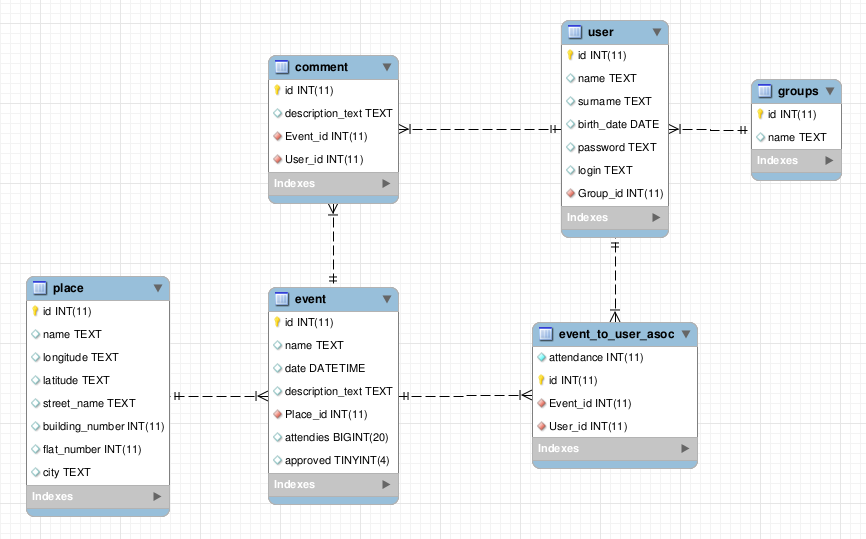
\includegraphics[width=\textwidth]{baza_mod.png}
  \caption{Schemat bazy danych dla aplikacji}
  \label{baza}
\end{center}
\end{figure}

\pagebreak
\section{Diagram klas aplikacji}
Poniższy diagram przedstawiony na rysunku \ref{klasy} pokazuje uproszczoną, abstrakcyjną strukturę aplikacji.
Przedstawione na nim zależności pokazują strukturę w jakiej zorganizowany został przepływ danych w naszej aplikacji.
Pozwala on na oddzielenie funkcjonalności związanej z bezpośrednią obsługą prostych zapytań do bazy danych, od bardziej skomplikowanych
operacji biznesowych.


\begin{figure}[!h]
\begin{center}
  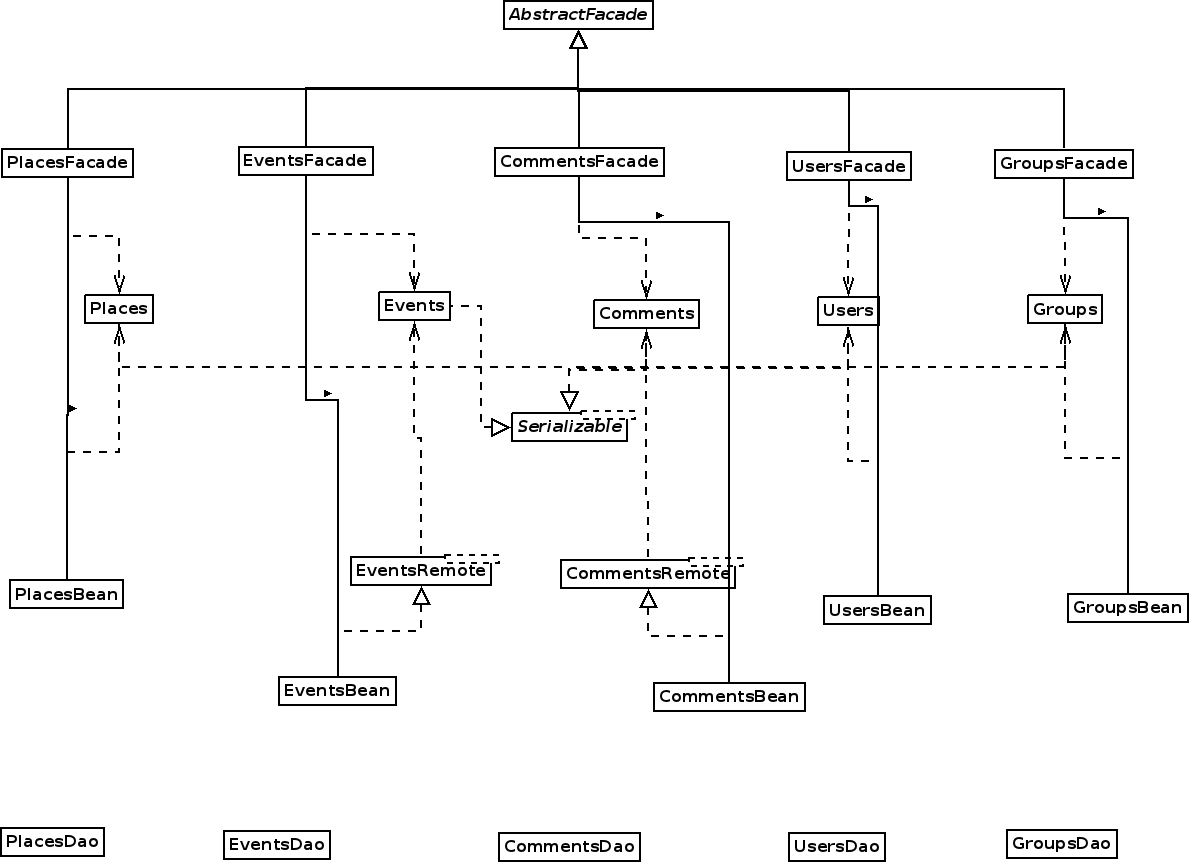
\includegraphics[width=\textwidth]{classDiagram.png}
  \caption{Diagram klas dla aplikacji}
  \label{klasy}
\end{center}
\end{figure}


\section{Dokumentacja aplikacji internetowej}

\subsection{Wykorzystane środowisko programistyczne}

Podczas tworzenia aplikacji zostały wykorzystane następujące narzędzia:
\begin{itemize}
 \item Zintegrowane środowisko programistyczne Netbeans w wersji 7.1.1
 \item MySQL Workbench do zarządzania bazą danych
 \item Serwer aplikacji Glassfish w wersji 3.1.2 (zintegrowany w naszym przypadku ze środowiskiem Netbeans)
 \item Meaven - narzędzie do automatyzacji budowy projektu
\end{itemize}

\subsection{Wykorzystane technologie}
Podczas tworzenia projektu zostały wykorzystane następujące technologie :
\begin{itemize}
 \item Język Java EE 6
 \item Baza danych MySQL
\end{itemize}


\subsection{Wykorzystywane biblioteki oraz frameworki}
Do stworzenia aplikacji wykorzystano następujące biblioteki oraz frameworki:
\begin{itemize}
 \item Biblioteka jdom w wersji 1.1
 \item Biblioteka Rome w wersji 1.0.0
 \item User Interface framework Primefaces w wersji 3.2 
 \item User Interface framework JavaServer Faces w wersji 2.0
\end{itemize}

Wszystkie zmieszczone na powyższej liście biblioteki lub frameworki zostały dodane do pliku konfiguracyjnego 
POM dla systemu budowania Meaven, dlatego też pobierane są automatycznie podczas pierwszego budowania projektu.
Nie wymagana jest żadna ręczna instalacja dodatkowych komponentów.

\subsection{Zmiany w stosunku do pierwotnej koncepcji}

Ponieważ podczas podczas tworzenia aplikacji, możliwe było skonfrontowanie realnych wymagań oraz możliwości wymaganiami 
założonymi na początku tworzenia projektu, poczyniono szereg zmian.
Zmiany te dotyczyły zarówno dodatkowych funkcjonalności jak i tych które zostały usunięte względem pierwotnego projektu.

\subsubsection{Funkcjonalności dodane podczas tworzenia projektu}
Podczas rozwijania projektu zostały dodatkowo zaimplementowane, nie wymienione w wymaganiach funkcjonalności:
\begin{enumerate}
 \item Możliwość dodawania komentarzy oraz ich podglądu dla wydarzeń, przez zalogowanego użytkownika.
 \item Możliwość potwierdzenia przyjścia na dane wydarzenie przez zalogowanego użytkownika.
 \item Możliwość podglądu tego ile osób i jacy użytkownicy mają zamiar przyjść na dane wydarzenie.
 \item Możliwość podglądu szczegółów zarówno wydarzenia jak i miejsca, w którym się odbywa.
 \item Możliwość edycji wydarzeń oraz miejsc przez administratora. 
\end{enumerate}
\subsubsection{Funkcjonalności zmodyfikowane podczas tworzenia projektu}
Podczas rozwijania projektu zostały zmodyfikowane lub usunięte następujące funkcjonalności:
\begin{enumerate}
 \item Możliwość podglądu wydarzeń najbliżej miejsca użytkownika - usunięcie zostało spowodowane zmianą charakteru aplikacji z ogólnej na 
wydarzenia ściśle związane z Wrocławiem, a także duży nakład pracy na implementacje tej funkcjonalności.
\item Możliwość przeszukiwania według miejsca została zmieniona z uwagi na brak sensu tego typu przeszukiwań w przypadku wydarzeń
dla jedynie Wrocławia, pozostawiono przeszukiwanie według daty wydarzenia.
\item Zmodyfikowano pobieranie informacji ze stron zewnętrznych, z parsowania stron na pobieranie informacji przy pomocy RSS.
\end{enumerate}


\subsection{Funkcjonalności aplikacji}
\subsubsection{Z punktu widzenia zwykłego użytkownika}

\subsubsection{Z punktu widzenia administratora}

\subsection{Widoki aplikacji}


\section{Dokumentacja aplikacji mobilnej}

\subsection{Wykorzystane środowisko programistyczne}

\subsection{Wykorzystane technologie}

\subsection{Wykorzystywane biblioteki oraz frameworki}

\subsection{Funkcjonalności aplikacji}

\subsection{Widoki aplikacji}


\end{document} 




